\documentclass[11pt,letterpaper]{article}
\usepackage[margin=0.85in]{geometry}
\usepackage[T1]{fontenc}
\usepackage{lmodern}
\usepackage{microtype}
\usepackage{amsmath,amssymb}
\usepackage{booktabs,tabularx,array}
\usepackage{enumitem}
\usepackage{xcolor}
\usepackage{tikz}
\usetikzlibrary{arrows.meta,positioning}
\usepackage[breaklinks=true,colorlinks=true,linkcolor=blue!50!black,
  citecolor=blue!50!black,urlcolor=blue!50!black]{hyperref}
\usepackage{url}
\setlist{nosep,leftmargin=*}
\setlength{\parskip}{0.35em}
\setlength{\parindent}{0pt}
\setlength{\emergencystretch}{2em}
\newcommand{\eV}{\,\mathrm{eV}}
\newcommand{\keV}{\,\mathrm{keV}}
\newcommand{\MeV}{\,\mathrm{MeV}}
\newcommand{\um}{\,\mu\mathrm{m}}
\newcommand{\nm}{\,\mathrm{nm}}
\newcommand{\doi}[1]{\href{https://doi.org/#1}{doi:\,#1}}
\newcolumntype{Y}{>{\raggedright\arraybackslash}X}

\title{Electron Energy Loss and Transport in Liquid Water\\
  \large A staged proposal and feasibility assessment for Jefferson Lab UITF}
\author{Working proposal for discussion}
\date{November 10, 2026}

\begin{document}
\maketitle

\begin{abstract}
We propose a staged program to measure electron energy-loss distributions, transmission, and scattering
in liquid water, with the scientific objective of constraining transport for electron kinetic energies
from $100\keV$ toward $1\keV$ and eventually below. The stated UITF beam range of
$0.5$--$7\MeV$ can support a useful apparatus and transport pilot, subject to confirmation of delivered
beam settings. It does not by itself provide a controlled $1\keV$ incident beam. Measuring electrons
that emerge at $1\keV$ after slowing in a thick target also does not directly determine bulk stopping
power at that energy. The recommended program combines a UITF pilot with development of a
monochromated low-energy source and an independently characterized liquid target. A direct bulk
stopping-power result at $1\keV$ is a conditional research objective; sub-keV bulk measurements remain
exploratory. The first deliverable should be calibrated spectra and an uncertainty assessment, with
stopping power reported only where its extraction is demonstrably identifiable.
\end{abstract}

\section{Scientific case and the meaning of the energy goal}

The repository README identifies reference data for electrons below $100\keV$, down to $1\keV$, as
the principal goal. The energy here is the electron kinetic energy $T$ in the liquid. It is distinct
from resolving an energy transfer $\Delta T=1\keV$ by a $500\keV$ incident electron. The latter would
measure high-energy energy loss, although it could be an important commissioning milestone.

Our proposed observables are energy and angle distributions as functions of incident energy, liquid
areal density, and controlled target conditions. In the regime where the interpretation is supported,
we seek the bulk electronic stopping power
\begin{equation}
  S_{\mathrm{el}}(T)=-\left\langle\frac{dT}{d\ell}\right\rangle_{\mathrm{electronic}},
  \qquad S_{\mathrm{el}}/\rho\quad\text{for the mass stopping power},
\end{equation}
where $\ell$ is actual trajectory length and $\rho$ is water density. A thickness scan measures a
dependence on slab thickness $t$, which is not automatically the same as a dependence on $\ell$.
Elastic scattering affects that distinction even when its direct energy transfer is negligible.

Kyriakou et al.\ compare five liquid-water track-structure codes from $20\eV$ to $100\keV$:
Geant4-DNA, PHITS-ETS, RITRACKS, NASIC, and PARTRAC~\cite{kyriakou}. Their Table~1 summarizes the
different collision models; their Fig.~12 compares stopping powers with ICRU Report~90 over
$1$--$100\keV$. The reported dispersion of transport observables is typically $5$--$15\%$ above
about $1\keV$, rising to $20$--$100\%$ below $100\eV$. This inter-code dispersion is evidence of
model dependence, rather than a confidence interval for the true stopping power.

The ICRU reference values in this comparison are calculations based on stopping-power theory, not
direct low-energy electron transmission measurements. Kyriakou et al.\ explicitly caution that
agreement above $1\keV$ does not validate sub-keV transport. They also describe experimental
liquid-water dielectric-response information used in model construction. Therefore the proposal
should state a shortage of direct, well-controlled liquid-phase transport benchmarks, rather than
claim that no liquid-water experimental information exists below $1\keV$.

\section{What the supplied papers establish}

\begin{table}[htbp]
\small
\begin{tabularx}{\linewidth}{@{}p{0.20\linewidth}YY@{}}
\toprule
Reference & Relevant contribution & Limit for this proposal \\
\midrule
Kyriakou et al.\ (2026)~\cite{kyriakou}
& Quantifies differences among liquid-water transport models and motivates independent benchmarks.
& A simulation comparison; Fig.~12 does not demonstrate an experimental method at $1\keV$. \\
\addlinespace
Bailey et al.\ (2015)~\cite{bailey}
& Analyzes ion-chamber perturbations and water--air stopping-power ratios for clinical electron
beams at $4$--$22\MeV$.
& Dose conversion and chamber corrections do not supply energy-resolved, low-energy electron
stopping-power measurements. \\
\addlinespace
Amin et al.\ (2011)~\cite{amin}
& Tests MOSFET relative dosimetry against other detectors for small clinical electron fields,
including $6$, $12$, $16$, and $20\MeV$ beams.
& Integrated dose response cannot reconstruct a $1\keV$ incident-electron loss distribution.
The PDF's publication year is 2011 despite the local filename saying 2010. \\
\bottomrule
\end{tabularx}
\caption{Interpretation of the three PDFs supplied with the project.}
\end{table}

The clinical dosimetry papers support using dose measurements as cross-checks at higher energy, and
emphasize detector perturbations. They do not justify selecting a MOSFET or an ion chamber as the
primary low-energy spectrometer. Kyriakou et al.\ also distinguish pathlength range, absorption range,
and CSDA range; these quantities must not be interchanged when interpreting transmission data.

Related work already addresses parts of the proposed problem. Muccignat et al.\ proposed electron
scattering from liquid microjets and studied extraction of collision information from simulated
energy-loss spectra~\cite{muccignat}. This is a particularly relevant prior feasibility study, not a
demonstration of precision bulk stopping power. Gadeyne et al.\ measured liquid-microjet
photoelectron spectra and tested low-energy scattering models and the escape
barrier~\cite{gadeyne,gadeyne-correction}. Such spectra provide important constraints but require a
transport and interface model. These precedents preclude an unqualified ``first low-energy electron
experiment in liquid water'' claim. Novelty should be assessed for the particular observable, energy
range, target metrology, and uncertainty achieved.

\section{Feasibility at UITF: facts and assumptions}

The starting specification supplied by the collaboration is a $0.5$--$7\MeV$ UITF electron beam,
with approximately $1\%$ energy precision and current potentially reaching microamperes. These are
planning inputs. ``Precision'' must be resolved into energy calibration, distribution width, and
time-dependent drift; one number cannot stand for all three.

The public UITF listing available during preparation gives operating points of $200\keV$ and
$8\MeV$, CW bunch repetition at $1497\,\mathrm{MHz}$ and subharmonics, spot sizes from hundreds of
micrometres to millimetres, and average currents of $100\,\mu\mathrm{A}$ at keV energy and
$100\,\mathrm{nA}$ at MeV energy~\cite{uitf}. These are advertised parameters, not a commitment for
this experiment, and do not establish continuous tuning from $0.5$ to $7\MeV$. Li et al.\ report
an earlier UITF irradiation-beamline design with an $8\MeV$ simulated beam and an rms energy spread
below approximately $74.5\keV$~\cite{li}. That result is configuration-specific, not a measurement of
the beam proposed here. The JLab UITF landing page is included as the facility entry point~\cite{jlab}.

\begin{table}[htbp]
\small
\begin{tabularx}{\linewidth}{@{}p{0.26\linewidth}YY@{}}
\toprule
Objective & Assessment & Essential condition \\
\midrule
Loss and scattering spectra at available $0.5$--$7\MeV$ settings
& Credible pilot at JLab.
& A matched beamline, target, calibrated spectrometer, and suitable low current. \\
\addlinespace
Resolve a $1\keV$ mean loss at $500\keV$
& Potentially feasible; unproven for the present apparatus.
& Adequate centroid precision, drift control, response calibration, and background rejection. \\
\addlinespace
Direct transport benchmarks at $10$--$100\keV$
& Plausible extension with additional source or beam preparation.
& Characterized electrons at the target and a suitably thin liquid geometry. \\
\addlinespace
Bulk $S_{\mathrm{el}}$ at $1\keV$
& Conditional research objective.
& Low-energy source, nanometre-scale target development, angular information, and demonstrated
separation of bulk and interface effects. \\
\addlinespace
Bulk $S_{\mathrm{el}}$ below $1\keV$
& High-risk exploratory objective.
& Evidence that interface, vapor, and multiple-scattering uncertainties permit a bulk inference. \\
\bottomrule
\end{tabularx}
\caption{The facility is a credible host for a staged program; its stated beam alone does not
establish the low-energy endpoint. All assessments are engineering judgments pending tests.}
\end{table}

\section{Quantitative constraints}

\subsection{Energy resolution, calibration, and statistical precision}

If $1\%$ denotes a beam distribution width, it corresponds to $5\keV$ at $500\keV$ and
$70\keV$ at $7\MeV$. A $1\keV$ shift is respectively $0.2\%$ and $0.014\%$ of the incident
energy. Such a shift need not be forbidden by a broader incident distribution: a stable mean can be
measured more precisely than its width. Under an ideal independent, Gaussian sampling assumption,
the uncertainty of the difference between two means is
\begin{equation}
  \sigma_{\Delta\bar T}=
  \sqrt{\frac{\sigma_0^2}{N_0}+\frac{\sigma_t^2}{N_t}}.
  \label{eq:centroid}
\end{equation}
For illustrative equal rms widths of $5\keV$ and equal counts $N$, reaching
$\sigma_{\Delta\bar T}=0.1\keV$ requires $N=5000$ per spectrum. This estimate excludes target
straggling, non-Gaussian tails, acceptance changes, and drift. If $1\%$ is instead an absolute
calibration uncertainty, Eq.~\ref{eq:centroid} does not reduce it. Interleave liquid and reference
measurements and monitor the incident distribution upstream of the target.

The low-energy goal is more demanding than ``$1\keV$ resolution.'' For a $1\keV$ incident electron,
a thin-target loss of $5\%$ is only $50\eV$. A $10\%$ measurement of that loss requires an uncertainty
around $5\eV$ in the corrected mean loss. A source/analyzer width of order $1$--$5\eV$ is an initial
design objective for loss-shape studies at this endpoint, subject to detailed optimization. The width,
energy zero, and stability each need their own specification.

\subsection{Target thickness, true path length, and interface contributions}

For nearly straight trajectories and small fractional losses, a useful starting relation is
\begin{equation}
  \langle\Delta T\rangle\simeq S_{\mathrm{el}}(T_0)t,
  \qquad \frac{\langle\Delta T\rangle}{T_0}\lesssim f,
  \qquad t\lesssim\frac{f T_0}{S_{\mathrm{el}}(T_0)},\quad f=0.05
  \label{eq:thin}
\end{equation}
as a proposed thin-target criterion. For scale only, assuming a mass collision stopping power of
$2\,\mathrm{MeV\,cm^2\,g^{-1}}$ and $\rho=1\,\mathrm{g\,cm^{-3}}$ gives
$S_{\mathrm{el}}=0.2\,\mathrm{keV\,\mu m^{-1}}$ and a $1\keV$ loss in $5\um$ of water. This is an
illustrative high-energy design estimate, not a tabulated value or a valid low-energy extrapolation.
Use evaluated values such as ESTAR for actual high-energy settings, with their documented limits,
and several track-structure models for low-energy target design~\cite{estar,kyriakou}.

At low energy, transmission requires targets on much smaller scales than conventional water cells.
Published windowless sheets span $250\nm$ to $2.5\um$ in one nozzle design~\cite{crissman}, while
gas-focused sheets have reached below $20\nm$, including a reported $16\pm2\nm$
measurement~\cite{koralek}. The latter is encouraging, but its relative thickness uncertainty is
already about $12.5\%$; it does not establish $3\%$ target metrology or a usable $1\keV$ thin-target
regime. Target requirements must be computed at each energy across competing models and checked
experimentally. Transmission alone is insufficient evidence for Eq.~\ref{eq:thin}.

Use measured transmission, angular broadening, energy distributions, and a thickness series together.
The following decomposition is only a diagnostic ansatz:
\begin{equation}
  \mu(t)=a_{\mathrm{interface}}+b_{\mathrm{bulk}}t+\delta_{\mathrm{transport}}(t).
  \label{eq:slope}
\end{equation}
It is justified only if the interface state remains comparable across thicknesses. In general,
surface transmission and multiple scattering are coupled to the bulk distribution and need a full
forward model. At finite thickness, the mean over detected transmitted electrons excludes stopped,
backscattered, and unaccepted electrons. Consequently
$\langle\Delta T\rangle_{\mathrm{detected}}/t$ is an acceptance-dependent quantity, not automatically
the unrestricted bulk stopping power. Secondary-electron multiplicity and the ambiguity of assigning
a primary after electron--electron collisions must also be treated consistently.

For a single-collision description, the desired bulk first moment has the schematic form
\begin{equation}
  S_{\mathrm{el}}(T)=n\!\int W\,
  \frac{d\sigma_{\mathrm{inel}}(T)}{dW}\,dW,
\end{equation}
including the relevant excitation channels. An experiment samples only a response-folded portion
of this kernel. Unmeasured angular regions and energy-loss tails can dominate corrections to the
first moment even when the main spectral peak is well measured.

\subsection{Why a thick degrader does not solve the low-energy problem}

Every stopping electron passes through low energies, but the depth and direction of that passage vary.
A water thickness chosen to reduce a $500\keV$ beam to a mean residual energy near $1\keV$ produces
large energy and angular spread, substantial loss of particles, and an emergent population biased
toward escape paths. The original electron can also be indistinguishable from secondaries. This
geometry can benchmark the full slowing-down and escape distribution, but does not isolate a
known-length $1\keV$ track segment.

A solid degrader followed by energy and angular selection could be evaluated as a source option.
Its usefulness depends on measured brightness, background, and stability after selection. It must
not be assumed to preserve the incident beam quality or yield a narrow low-energy beam for free.

Electrostatic deceleration is another possible development, not an established UITF capability.
Reducing $500\keV$ to $1\keV$ requires a retarding-potential magnitude near $499\,\mathrm{kV}$;
reducing $7\MeV$ to $1\keV$ would require nearly $7\,\mathrm{MV}$. Conservative deceleration by a
common potential does not remove the absolute energy spread: a hypothetical $5\keV$ initial rms
width is still inappropriate for a $1\keV$ output without selection or other beam manipulation.
Retarding optics also restrict transverse phase space and can reflect particles. A dedicated gun is
the recommended baseline for the low-energy stage.

\subsection{Rate and deposited power}

The electron rate is $\dot N=I/e=6.24\times10^6\,\mathrm{s^{-1}}$ at $1\,\mathrm{pA}$. For an
illustrative accepted probability $\eta=10^{-4}$ per incident electron in a selected measurement,
\begin{equation}
  R=624\,\mathrm{s^{-1}}
    \left(\frac{I}{1\,\mathrm{pA}}\right)
    \left(\frac{\eta}{10^{-4}}\right).
\end{equation}
The factor $\eta$ includes scattering probability, transport, solid angle, energy acceptance, and
efficiency; it has not been measured for this design. At $10^3$ accepted counts/s, a spectrum with
$10^6$ total counts takes about 17 minutes before scans, references, and dead time. Counts in rare
tails, rather than the total alone, may determine run time. Picoampere-to-low-nanoampere studies
are a reasonable starting request, but UITF stability and current monitoring in that range require
confirmation. Available maximum current is not the key figure of merit.

Beam power is $P_{\mathrm{beam}}=I T_0/e$. At $1\,\mu\mathrm{A}$ this is $0.5\,\mathrm{W}$ at
$500\keV$ and $7\,\mathrm{W}$ at $7\MeV$. A thin target instead absorbs approximately
$P_{\mathrm{water}}=I\langle\Delta T\rangle/e$: a $1\keV$ mean loss gives $1\,\mathrm{mW}$ at
$1\,\mu\mathrm{A}$ and $1\,\mathrm{nW}$ at $1\,\mathrm{pA}$. Even low total power does not
guarantee negligible local radiolysis. Scan current and flow speed and require stable spectra and
target properties. The transmitted beam needs a separate, appropriately rated dump.

\section{Recommended experimental architecture}

\begin{figure}[htbp]
\centering
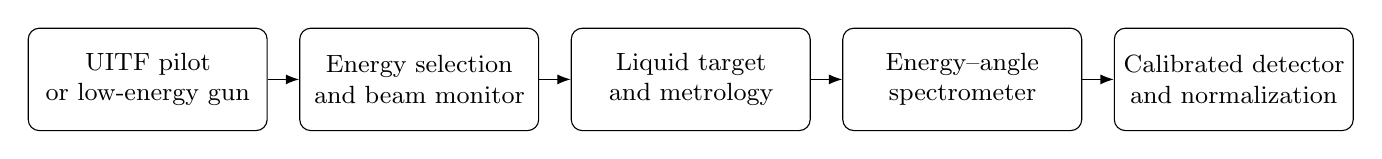
\begin{tikzpicture}[node distance=4mm,>=Latex,
  box/.style={draw,rounded corners,align=center,text width=28mm,minimum height=13mm,font=\small}]
  \node[box] (source) {UITF pilot\\or low-energy gun};
  \node[box,right=of source] (incident) {Energy selection\\and beam monitor};
  \node[box,right=of incident] (water) {Liquid target\\and metrology};
  \node[box,right=of water] (analyzer) {Energy--angle\\spectrometer};
  \node[box,right=of analyzer] (detector) {Calibrated detector\\and normalization};
  \draw[->] (source) -- (incident);
  \draw[->] (incident) -- (water);
  \draw[->] (water) -- (analyzer);
  \draw[->] (analyzer) -- (detector);
\end{tikzpicture}
\caption{Common measurement concept. The UITF pilot and the dedicated low-energy stage require
different source optics and likely different analyzers; the diagram does not imply one instrument
can cover the entire energy range.}
\end{figure}

\subsection{Stage A: UITF apparatus and transport pilot}

Use the lowest delivered energy that the facility can support, followed by one or more higher-energy
settings. A windowless, flowing liquid sheet is the preferred target concept. A membrane liquid cell
is an alternative for commissioning if the membrane and water contributions can be characterized
separately. Entrance and exit windows, gas paths, and detector entrance layers must be included in
the response model.

Use upstream energy selection or a beam spectrometer to characterize the incident distribution.
Analyze outgoing electrons with a calibrated magnetic spectrometer and a position-sensitive
detector, with explicit energy and angular acceptance. Map the response using the beam without
liquid and appropriate calibration measurements. A bulk silicon detector or calorimeter can help
commission the beam, but should not be assigned sub-keV resolution without evidence including
entrance-layer losses, electron backscatter, and detector response tails.

Measure at least three independently characterized nonzero thicknesses and a reference configuration
at each chosen energy. Record energy spectra, angular distributions or angular scans, transmission,
incident charge, target thickness and position, and beam stability. Seek a small-loss benchmark
including, if achievable, a $1\keV$ mean loss at an available high-energy setting. This is a useful
pilot result even if it has little sensitivity to the sub-keV collision models.

An optional low-energy emission arm can measure angle-resolved electron yields from the irradiated
liquid. Report these as escape spectra per incident charge, with a defined energy zero and angular
acceptance. Any inference about transport inside water must account for production, scattering,
the liquid--vacuum barrier, and surface potentials.

\subsection{\texorpdfstring{Stage B: controlled $100$ to $1\keV$ incident electrons}
  {Stage B: controlled 100 to 1 keV incident electrons}}

Develop or bring a dedicated variable-energy electron source, with an initial sequence such as
$100$, $50$, $20$, $10$, $5$, $2$, and $1\keV$. These are proposed measurement points, not
UITF settings. A conventional high-voltage electron gun and suitable selection optics can be
assessed for the upper part of the range; the endpoint requires tighter control of energy and stray
fields. The low-energy end station could share target technology and analysis with Stage~A while
operating independently of the accelerator.

Select an electrostatic energy analyzer, with retardation optics where appropriate, and a calibrated
electron detector. Measure its transmission versus energy and angle. A retarding-field measurement
alone generally mixes energy and emission direction and needs angular control. Avoid a requirement
for a single analyzer or detector to perform equally well at eV and MeV energies.

For each energy, select thicknesses using Eq.~\ref{eq:thin}, predicted angular broadening, and
transmission across multiple models. Start where the target is demonstrably thin enough and descend
only after closure tests. A $250\nm$ or even $20\nm$ target should not be presumed suitable at
$1\keV$ simply because it is called ultrathin. If no accessible thickness permits a bulk inference,
switch the deliverable at that energy to measured transport spectra with explicit interface
sensitivity and defer a stopping-power claim.

Time of flight is optional rather than the baseline. For scale, a $1\keV$ electron takes about
$53\,\mathrm{ns}$ to cross $1\,\mathrm{m}$ in vacuum, whereas the nominal $1497\,\mathrm{MHz}$
bunch spacing is about $0.67\,\mathrm{ns}$. UITF time-of-flight measurements would therefore require
suitable pulse selection or a demonstrated method to resolve bunch ambiguity, as well as verified
timing and flight-path calibration.

\subsection{Stage C: sub-keV exploration}

After successful $1$--$2\keV$ measurements, explore $500$, $200$, and $100\eV$ only as justified
by source and target performance. At these energies the escaped spectrum increasingly depends on
interface transmission, electrostatic potentials, and the vapor environment. At still lower energies,
vibrational losses, attachment, and the definition of the modeled electron state become important.
Keep this distinct from a promise to measure an unrestricted bulk stopping power. A surface-sensitive
observable can still be scientifically useful if its geometry, energy scale, and model dependence
are reported.

\section{Target metrology and control measurements}

Use fresh, flowing water with measured temperature, conductivity, and purity. Determine the local
thickness distribution over the beam spot, rather than a nozzle nominal thickness. Combine optical
interferometry where sensitive with a second method suitable for the thinnest targets, for example
calibrated absorption. Electron attenuation alone yields a thickness only after assuming a mean
free path, so it cannot be the sole independent calibration when those collision models are under test.

Characterize evaporative cooling, possible freezing, sheet motion, and the gas or vapor column in
the actual beam path. Gas-focused sheets also introduce a sheath gas. The target chamber requires
differential pumping, a liquid catcher, and isolation from the accelerator vacuum; compatibility
with the UITF installation is an engineering prerequisite. Free liquid surfaces cannot independently
scan arbitrary pressure and temperature without affecting evaporation and stability. Begin with one
documented thermodynamic state; add temperature and pressure scans only after the baseline works.

At low energy, monitor streaming and charging potentials and the analyzer energy reference. A few
volts of potential shift correspond to several eV of electron energy, material for the $1\keV$
endpoint and dominant in some lower-energy measurements. Adding electrolyte can reduce charging
but changes the target composition; any such solution requires separate characterization and cannot
silently stand in for pure water.

Essential controls are:
\begin{enumerate}
  \item Interleaved incident-beam and reference spectra, including liquid removed from the beam.
  \item Vapor and sheath-gas characterization at matched conditions as closely as possible. Simply
    turning off the jet also changes the gas load and is not a complete background subtraction.
  \item Empty-cell or support references if membranes are used, with checks for wetting-induced
    changes. Membrane subtraction is not assumed to be a simple additive correction.
  \item Beam-position, angular-acceptance, thickness, current, and flow scans to expose correlated
    biases and beam-induced changes.
  \item Detector-efficiency, dead-time, pile-up, and low-energy threshold measurements, including
    calibration of response tails and magnetic/electric stray-field effects.
\end{enumerate}

\section{Analysis strategy and uncertainty requirements}

The primary data product is the normalized detected distribution in outgoing kinetic energy and
angle, accompanied by transmission and the incident-beam distribution. Fit measured spectra with a
response-folded forward prediction. Schematically,
\begin{equation}
  C_i = N_{\mathrm{inc}}\!\int dT_0\,f_0(T_0)
  \int dT\,d\Omega\, R_i(T,\Omega)\,
  K(T,\Omega\mid T_0,t,\boldsymbol{\theta})+B_i .
  \label{eq:forward}
\end{equation}
Here $K$ is the emergent electron yield per incident electron, including transport, secondaries,
interfaces, and target-thickness distribution; $R_i$ includes acceptance, efficiency, and bin response;
$B_i$ describes residual background. Nuisance parameters $\boldsymbol{\theta}$ include independently
constrained geometry, potentials, and material state. Normalization must allow yield and multiplicity,
rather than forcing every incident electron to produce one detected electron.

Compare at least two substantially different collision-model choices and scan their elastic and
inelastic components separately. Record exact software versions, model options, transport cutoffs,
and material assumptions. Standard condensed-history transport may be suitable for the high-energy
pilot but is not an independent validation of sub-keV physics. In the low-energy region, track-structure
models should predict observables; they must not provide an unexamined correction that predetermines
the extracted stopping power.

Before fitting real data, generate synthetic spectra with one model and analyze them with another.
Vary surface potentials, elastic scattering, target thickness, and lost angular/energy tails. Establish
which bulk parameters are actually constrained by the planned measurements. If equally acceptable
fits give materially different stopping powers, publish the transport data and the resulting range of
inferences instead of a model-independent stopping-power claim.

\begin{table}[htbp]
\small
\begin{tabularx}{\linewidth}{@{}p{0.32\linewidth}p{0.15\linewidth}Y@{}}
\toprule
Contribution to an inferred $S$ & Illustrative goal & Verification \\
\midrule
Corrected mean energy loss & $3\%$ & Statistics, energy scale, drift, and response-tail propagation. \\
Effective liquid path/areal density & $3\%$ & Independent thickness map, density, and trajectory checks. \\
Angular acceptance and missing yield & $3\%$ & Angular scans and measured response constraints. \\
Background and interface correction & $2\%$ & References and thickness/geometry variation. \\
Residual transport inference & $3\%$ & Cross-model closure and alternative parameterizations. \\
\bottomrule
\end{tabularx}
\caption{An example target budget, not demonstrated performance. If independent, these entries
combine to about $6.3\%$. Correlations and unconstrained model biases can make the total larger.}
\end{table}

For a $50\eV$ mean loss, the $3\%$ loss term in this budget corresponds to $1.5\eV$ uncertainty;
it is substantially stricter than the earlier $10\%$ loss example. No entry is known to be achieved
at $1\keV$. The reported $16\pm2\nm$ liquid-sheet example alone exceeds this target thickness
budget. For a benchmark intended to distinguish differences at the $20\%$ scale, aim initially for
combined uncertainty below approximately $7$--$10\%$, while recognizing that model differences
depend on the particular measured observable. Forward predictions should show separation in
measured bins after all nuisance parameters are varied.

\section{Work plan, decision criteria, and resources}

\begin{table}[htbp]
\small
\begin{tabularx}{\linewidth}{@{}p{0.16\linewidth}YY@{}}
\toprule
Phase & Concrete output & Criterion for proceeding \\
\midrule
Design and simulation
& Confirmed facility parameter sheet; target and analyzer designs; synthetic-data study.
& At least one accessible configuration separates relevant transport predictions after realistic
nuisance variations. Otherwise revise the observable or apparatus. \\
\addlinespace
Bench commissioning
& Independent target metrology, liquid/vapor controls, calibrated energy and angle response.
& Stable liquid state and a quantified uncertainty budget; selected targets satisfy the intended
transmission and loss conditions. \\
\addlinespace
UITF pilot
& Spectra and scattering data at available settings, with thickness and current scans.
& Reproducible reference-corrected results and acceptable beamline/target operation. This validates
the apparatus, not low-energy collision models. \\
\addlinespace
$10$--$100\keV$ campaign
& Transport benchmarks with a characterized low-energy source.
& Closure on independent configurations; corrections smaller than the physics discrimination sought. \\
\addlinespace
$1$--$5\keV$ development
& Thickness and angle series; an identifiable bulk result or a documented transport-only result.
& Source, target, interface, and missing-yield uncertainties meet the stated endpoint requirements. \\
\addlinespace
Sub-keV study
& Exploratory spectra and a quantified assessment of bulk sensitivity.
& Proceed only where bulk and interface effects can be distinguished; otherwise retain the
surface-sensitive measurement as the deliverable. \\
\bottomrule
\end{tabularx}
\caption{Proposed sequence. No beam time, equipment availability, cost, or schedule is assumed approved.}
\end{table}

The initial resource request should cover accelerator liaison and beam characterization, a liquid-jet
and vacuum specialist, electron-spectroscopy expertise, target metrology, detector/data-acquisition
support, and transport analysis. Equipment needs include a characterized liquid-sheet system,
vacuum isolation and pumping, an upstream monitor, outgoing analysis optics, a detector, and
calibration hardware. The dedicated low-energy source and electrostatic analyzer are additional
development items unless an identified collaborator already provides them. Cost and schedule should
follow a component inventory and the synthetic-data study, rather than precede them.

Suitable discussions include UITF staff for delivered beam and optics, liquid-sheet developers for
target feasibility, and low-energy electron scattering/track-structure groups for observables and
independent predictions. The README identifies L.\ Braby as a possible scientific adviser. No
participation or collaboration is assumed, and no contacts have been made in preparing this proposal.

\section{Questions to settle with the facility and collaboration}

\begin{enumerate}
  \item Which energies can be delivered at the experimental target, especially near $500\keV$?
    Can the gun-only beam be accessed, and what changes are needed between settings?
  \item Does the stated $1\%$ describe rms spread, FWHM, energy calibration, reproducibility, or
    another quantity? What are the measured tails and drift over a thickness scan?
  \item What currents, spot sizes, divergence, and monitoring precision are available in the proposed
    low-current mode? What pulse patterns and subharmonics can be provided if timing is needed?
  \item Can a differentially pumped liquid target be installed at the available location, with adequate
    spectrometer space and a defined vacuum interface? Which equipment is already available?
  \item Is the collaboration willing to make a dedicated low-energy source part of the program,
    potentially with an off-beamline end station, or must all data use the existing UITF beam?
  \item Is the first success criterion a published transport benchmark, or specifically a bulk
    stopping-power value? What combined uncertainty would make that result useful?
\end{enumerate}

\section{Recommendation}

Proceed with a limited design and apparatus study at JLab. UITF offers a credible platform for a
high-energy pilot and for testing liquid targets, beam normalization, and electron analysis. The
scientific goal of reaching $1\keV$ electron kinetic energy is plausible only as a staged development
program with controlled low-energy beam preparation and demanding target metrology. It cannot be
promised from the stated $0.5$--$7\MeV$ beam alone. A result below $1\keV$ should remain a stretch
objective until measurements demonstrate that bulk transport is distinguishable from interface and
escape effects. Preserve publishable energy--angle spectra and transmission data at every stage,
even where a unique stopping-power extraction is not justified.

\appendix
\section{Sources, provenance, and rebuilding}

The three local PDFs and the project README were reviewed directly. Online primary literature and
facility listings were consulted on November 10, 2026. Public operating parameters may change;
facility confirmation is required. Numerical examples labeled illustrative are calculations for
planning, not measured performance. ICRU Report~90 is discussed as described by Kyriakou et al.;
its original full report was not independently reviewed. No new transport simulation, instrument
optimization, or beam test has been performed for this document.

This source has an embedded bibliography and requires no external figures or bibliography database.
Build with \texttt{meson setup build} followed by \texttt{meson compile -C build}; the output is
\texttt{build/proposal.pdf}. Copy that PDF to the repository root when updating the tracked snapshot.

\begin{thebibliography}{99}

\bibitem{kyriakou}
I.\ Kyriakou et al., ``Intercomparison of low-energy electron transport calculations by different
Monte Carlo track-structure simulation codes,'' \emph{Phys.\ Med.\ Biol.}\ \textbf{71}, 085009 (2026).
\doi{10.1088/1361-6560/ae5758}.
Local supplied PDF; especially Table~1, Secs.~2.3 and 3.3, Fig.~12, and the discussion.

\bibitem{bailey}
M.\ Bailey, D.\ R.\ Shipley, and J.\ W.\ Manning, ``Roos and NACP-02 ion chamber perturbations
and water-air stopping-power ratios for clinical electron beams for energies from 4 to 22 MeV,''
\emph{Phys.\ Med.\ Biol.}\ \textbf{60}, 1087--1105 (2015).
\doi{10.1088/0031-9155/60/3/1087}. Local supplied PDF.

\bibitem{amin}
Md N.\ Amin, R.\ Heaton, B.\ Norrlinger, and M.\ K.\ Islam, ``Small field electron beam dosimetry
using MOSFET detector,'' \emph{J.\ Appl.\ Clin.\ Med.\ Phys.}\ \textbf{12}(1), 50--57 (2011),
article 3267. \doi{10.1120/jacmp.v12i1.3267}. Local supplied PDF; received and accepted in 2010.

\bibitem{muccignat}
D.\ L.\ Muccignat et al., ``Simulating the Feasibility of Using Liquid Micro-Jets for Determining
Electron--Liquid Scattering Cross-Sections,'' \emph{Int.\ J.\ Mol.\ Sci.}\ \textbf{23}, 3354 (2022).
\doi{10.3390/ijms23063354}.

\bibitem{gadeyne}
T.\ Gadeyne, P.\ Zhang, A.\ Schild, and H.\ J.\ W\"orner, ``Low-energy electron distributions from
the photoionization of liquid water: a sensitive test of electron mean free paths,''
\emph{Chem.\ Sci.}\ \textbf{13}, 1675--1692 (2022). \doi{10.1039/D1SC06741A}.

\bibitem{gadeyne-correction}
T.\ Gadeyne et al., correction to Ref.~\cite{gadeyne}, \emph{Chem.\ Sci.}\ \textbf{16}, 6522 (2025).
\doi{10.1039/D5SC90072G}. Corrects the lower-panel horizontal scale in Fig.~4 from
$0$--$50\eV$ to $0$--$1\eV$; the authors state that the conclusions are unaffected.

\bibitem{uitf}
beamNetUS, ``UITF---Upgraded Injector Test Facility,'' facility description and beam parameters.
\url{https://www.beamnetus.org/uitf}. Accessed November 10, 2026.

\bibitem{li}
X.\ Li et al., ``Design of a 10 MeV Beamline at the Upgraded Injector Test Facility for e-Beam
Irradiation,'' \emph{Proc.\ IPAC2021}, 3232--3235 (2021), paper WEPAB254.
\doi{10.18429/JACoW-IPAC2021-WEPAB254}.
\url{https://proceedings.jacow.org/ipac2021/papers/wepab254.pdf}.

\bibitem{jlab}
Jefferson Lab, UITF facility landing page, supplied by the collaboration.
\url{https://www.jlab.org/accelerator/uitf}. Accessed November 10, 2026.
The retrievable page did not provide a complete beam-parameter specification.

\bibitem{estar}
NIST, ESTAR: stopping powers and ranges for electrons.
\url{https://physics.nist.gov/PhysRefData/Star/Text/ESTAR.html}.
The online calculation accepts kinetic energies starting at $0.001\MeV$; this input limit does not
constitute experimental validation at $1\keV$. Accessed November 10, 2026.

\bibitem{crissman}
C.\ J.\ Crissman et al., ``Sub-micron thick liquid sheets produced by isotropically etched glass
nozzles,'' \emph{Lab Chip}\ \textbf{22}, 1365--1373 (2022). \doi{10.1039/D1LC00757B}.

\bibitem{koralek}
J.\ D.\ Koralek et al., ``Generation and characterization of ultrathin free-flowing liquid sheets,''
\emph{Nat.\ Commun.}\ \textbf{9}, 1353 (2018). \doi{10.1038/s41467-018-03696-w}.
The online article incorporates a 2019 correction to its absorbance equation.

\end{thebibliography}
\end{document}
